\documentclass[10pt,a4paper]{article}
\usepackage[latin1]{inputenc}
\usepackage[spanish]{babel}
\usepackage{amsmath}
\usepackage{amsfonts}
\usepackage{amssymb}
\usepackage{graphicx}
\usepackage{textcomp}
\author{Santiago Videla - Francisco Javier Herrero}
\title{Pr\'actico Especial II: Selecci\'on de Distribuciones de Probabilidad}
\pagestyle{headings}
\begin{document}
\maketitle
\newpage
\tableofcontents
\newpage

\section{Independencia estad\'istica}

\paragraph{}
A partir de los datos obtenidos en la simulaci\'on, se corroboro la
independencia de los mismos mediante un \textit{scatter plot} como se puede ver
en la Figura~\ref{scatter}. Los valores observados, se distribuyen de manera
aleatoria en el primer cuadrante del plano, lo que indica la independencia de
los datos.

\begin{figure}
  \centering
  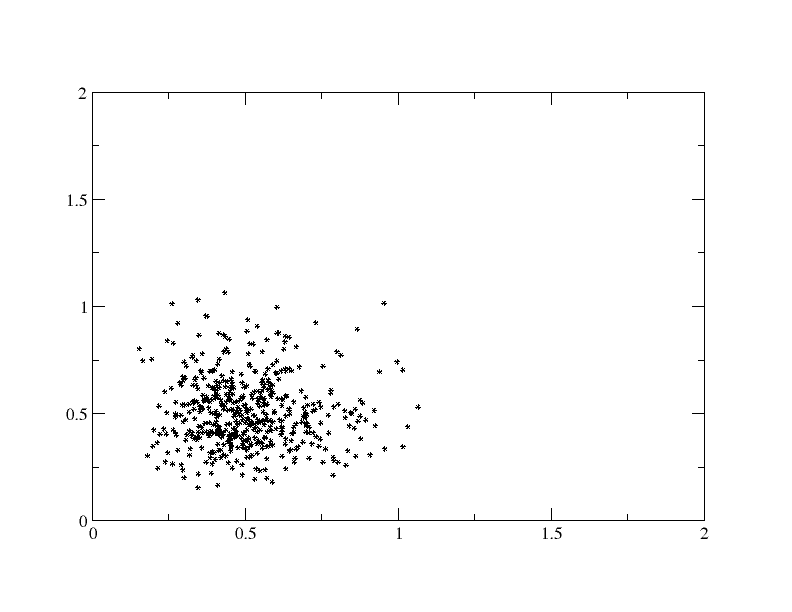
\includegraphics[scale=0.5]{scatter.png} 
  \caption{Scatter}
  \label{scatter}
\end{figure}

\section{Estad\'istica}

\begin{itemize}
  \item \textbf{M\'inimo:} 0.153672
  \item \textbf{M\'aximo:} 1.064818
  \item \textbf{Mediana:} 0.491458
  \item \textbf{Media:} 0.509307
  \item \textbf{1er. cuartil}: 0.398686
  \item \textbf{2do. cuartil}: 0.600152
  \item \textbf{Varianza:} 0.026880
  \item \textbf{Asimetria:} 0.652167
\end{itemize}

Observando el valor de asimetr\'ia, la varianza y el boxplot de la figura \ref{boxplot}, 
se puede observar que los datos estan desplazados hacia la izquierda y altamente concentrados.


\begin{figure}
  \centering
  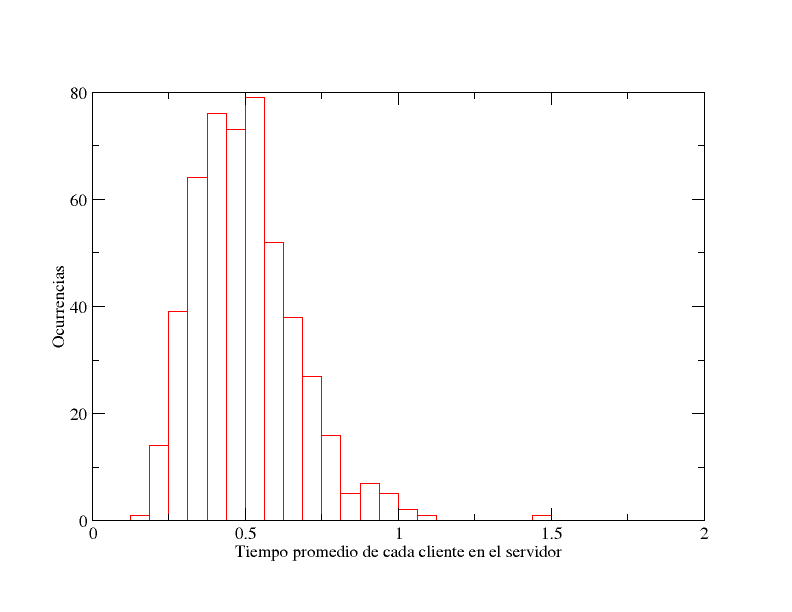
\includegraphics[scale=0.5]{histogram.png} 
  \caption{Histograma}
  \label{histogram}
\end{figure}

\begin{figure}
  \centering
  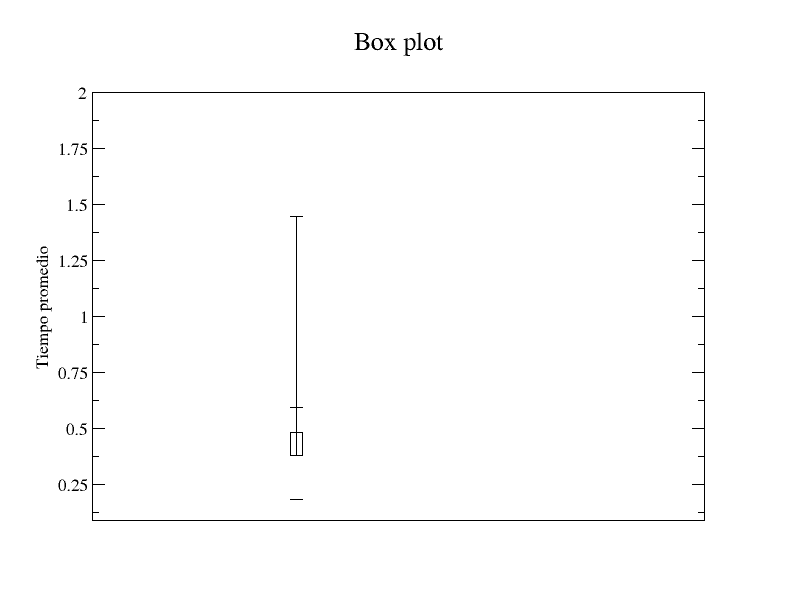
\includegraphics[scale=0.5]{boxplot.png} 
  \caption{Boxplot}
  \label{boxplot}
\end{figure}

\section{Estimacion de par\'ametros}

\begin{itemize}
  \item N($\mu$, $\sigma^{2}$): \\
    $\mu = 0.509307$ \\
    $\sigma^{2} = 0.026826$
  \item LN($\mu$, $\sigma^{2}$): \\
    $\mu = -0.727032$ \\
    $\sigma^{2} = 0.108136$
  \item Gamma($\alpha$, $\beta$): \\
    $\alpha = 9.789000$ \\
    $\beta = 0.052028$
\end{itemize}

\section{Bondad de los ajustes}

\paragraph{Comparaci\'on de frecuencias:}
En las Figura~\ref{freq-normal}, se comparan los datos muestrales con la
distribuci\'on normal. En la Figura~\ref{freq-lognormal}, se realiza la misma
comparaci\'on con la distribuci\'on LogNormal. Finalmente, en la
Figura~\ref{freq-gamma}, se compara con la distribucion Gamma. De estos
graficos podemos suponer que la distribuci\'on Gamma es la que mejor se ajusta
a los datos.

Luego, se realizaron las pruebas de hipotesis tanto usando $\chi^2$ como
Kolmogorov Smirnov y se presentan los resultados obtenidos en el
cuadro~\ref{estimators}

\begin{figure}
  \centering
  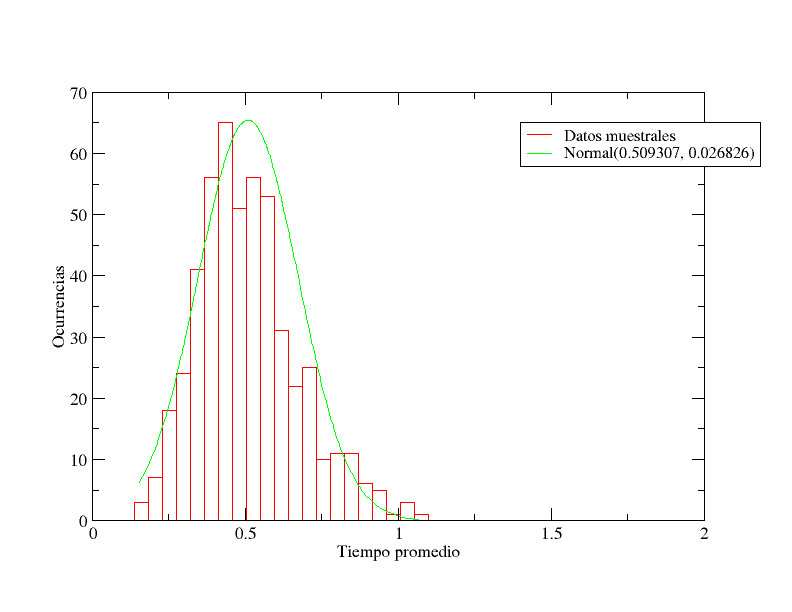
\includegraphics[scale=0.5]{freq-normal.png} 
  \caption{Muestra/Normal}
  \label{freq-normal}
\end{figure}

\begin{figure}
  \centering
  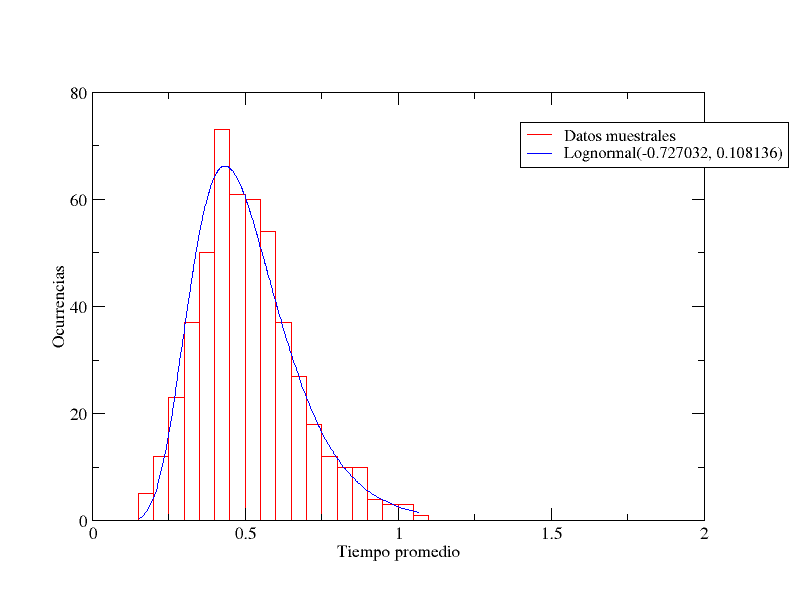
\includegraphics[scale=0.5]{freq-lognormal.png} 
  \caption{Muestra/LogNormal}
  \label{freq-lognormal}
\end{figure}

\begin{figure}
  \centering
  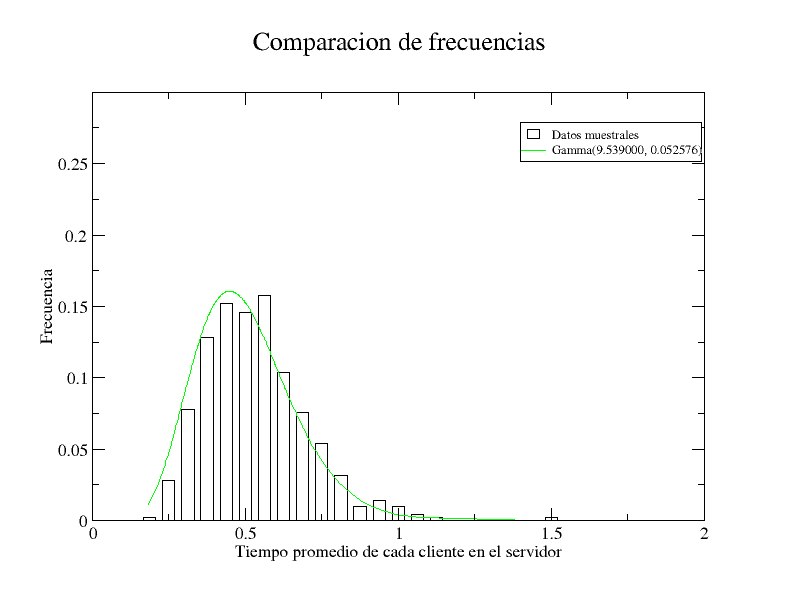
\includegraphics[scale=0.5]{freq-gamma.png} 
  \caption{Muestra/Gamma}
  \label{freq-gamma}
\end{figure}

\begin{table}[ht]
\caption{Resultado de las estimaciones de p-valor}
\centering
\begin{tabular}{c c c c c}
\hline\hline
Distribuci\'on & $T_0$ & $\chi^2$ & $D_0$ & p-valor (K-S)\\ [0.5ex]
\hline
Normal & 68.832119 & 0.000001 & 0.055291 & 0.109000 \\
LogNormal & 26.257540 & 0.240789 & 0.033047 & 0.651000 \\
Gamma & 18.147321 & 0.697219 & 0.025335 & 0.900000 \\
\hline
\end{tabular}
\label{estimators}
\end{table}

\section{Conclusiones}

Observando las figuras comparativas en primera instancia Gamma parece ser la que mejor se ajusta a distribuci\'on simulada, sin embargo es muy 
sutil la diferencia. 
Analizando los valores de $\chi^2$ y el p-valor a partir de Kolmogorov Smirnov (K-S) en el cuadro \ref{estimators} se puede observar que la probabilidad
de ser la distribuci\'on normal la adecuada es muy baja.
En el caso de la LogNormal, la $\chi^2$ genera un n\'umero mas razonable, que en K-S se incrementa notablemente a un 65\% de probabilidades de ser cierta
la hip\'otesis.
Finalmente, se verifica que la distribuci\'on Gamma se ajusta mucho mejor, dando un 70\% en $\chi^2$ y 90\% en K-S. 

\end{document}
